
\section{Overview of Human Action Recognition}
\begin{frame}{Overview of Human Action Recognition}
    Human action recognition can be divided into action classification and action detection.
    \begin{itemize}
        \item Action classification is the analysis of a segmented video containing only a single action that must be classified into a defined action category (early).
        \item Action detection detects the start and end times of each action in the video, locates their position in space, and identifies the action category (more challenging).
    \end{itemize}
\end{frame}

\begin{frame}{Overview of Human Action Recognition}
    Techniques can be categorized into the following four classes of action semantics from low to high:
    \begin{itemize}
        \item Primitive action recognition (waving, lifting a foot, bending).
        \item Single-person action recognition (walking, punching, jumping).
        \item Interaction recognition (playing an instrument, carrying a knife). It has received \textbf{more attention in recent years}.
        \item Group action recognition (parade, group meeting). It is \textbf{still in its infancy}.
    \end{itemize}
\end{frame}

\section{Applications}
\begin{frame}{Applications}
    Human action recognition has a wide range of a applications:

    \begin{itemize}
        \item Intelligent video surveillance. [1]
        \item Environmental home monitoring. [2]
        \item Video storage and retrieval. [3,4]
        \item Intelligent human–machine interfaces. [5,6]
        \item Identity recognition [7].
    \end{itemize}
\end{frame}

\section{Type of Dataset}
\begin{frame}{Type of Dataset}
    Most reviews of human action recognition are limited to approaches based on specific data:

    \begin{itemize}
        \item RGB data.
        \item Depth data.
        \item Skeleton data.
    \end{itemize}
\end{frame}

\begin{frame}{Type of Dataset}
    Skeleton and RGB and Depth sample frames from the NTU RGB+D Human Activity Dataset \cite{shahroudy2016ntu}.
    \begin{multicols}{2}
        \begin{figure}[htp]
            \centering
            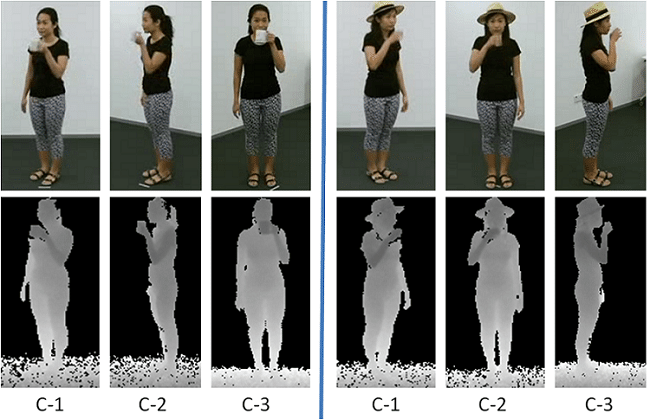
\includegraphics[height=3cm]{images/v1survey/depth_data_ex.png}
            \caption{Depth data}
            \label{fig:depth_data_ex}
        \end{figure}
        \begin{figure}[htp]
            \centering
            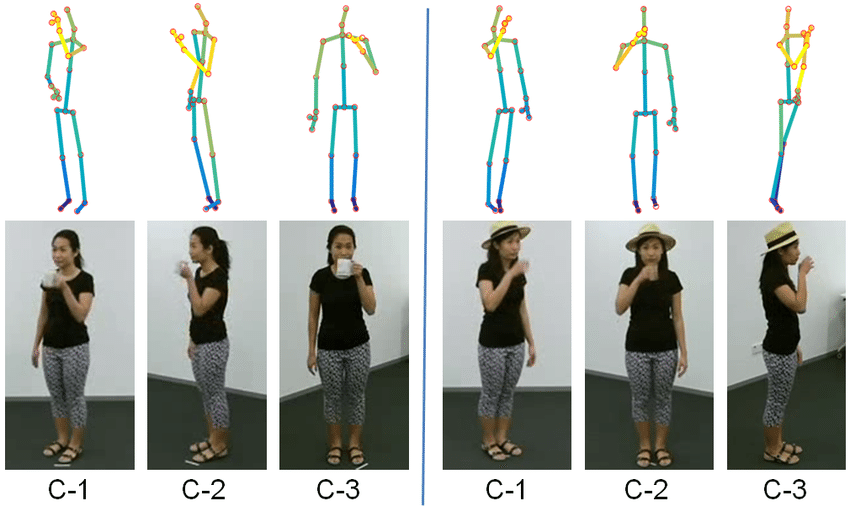
\includegraphics[height=3cm]{images/v1survey/skeleton_data_ex.png}
            \caption{Skeleton data}
            \label{fig:skeleton_data_ex}
        \end{figure}
    \end{multicols}
\end{frame}

\section{Feature representation}
\begin{frame}{Feature representation}
    \begin{itemize}
        \item The problem of feature representation in HAR is extended from two-dimensional space to three-dimensional space-time.
        \item In recent years, many kinds of action representation methods have been proposed:
              \begin{enumerate}
                  \item Action Features for RGB Data.
                  \item Action Features for Depth and Skeleton Data.
                  \item Feature Fusion methods.
              \end{enumerate}
    \end{itemize}
\end{frame}

\begin{frame}{Handcrafted Action Features (RGB)}
    \begin{itemize}
        \item<1-> Spatiotemporal volume-based action representation methods (\href{https://web.cse.ohio-state.edu/~davis.1719/CVL/Research/MHI/mhi.html}{motion history image, motion energy image}) \cite{li2011human}.
              \only<1>{
                  \begin{figure}[htp]
                      \centering
                      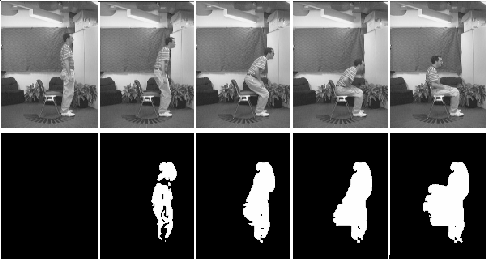
\includegraphics[height=2cm, width=7cm]{images/v1survey/mei.png}
                      \caption{Motion history image}
                  \end{figure}
                  \begin{figure}[htp]
                      \centering
                      \includegraphics<1>[height=2cm, width=7cm]{images/v1survey/mhi.png}
                      \caption{Motion energy image}
                  \end{figure}
              }
              % [Global features] The camera is fixed  -> background subtraction techniques
              % -> shape information (silhouettes and contours) -> key template matrix -> matching
        \item<2-> STIP-based methods (Feature descriptors: SIFT, HOG) \cite{nguyen2014stap} \cite{dalal2005histograms}.
              % [Local features] key region of movement change.
              \only<2>{
                  \begin{figure}[htp]
                      \centering
                      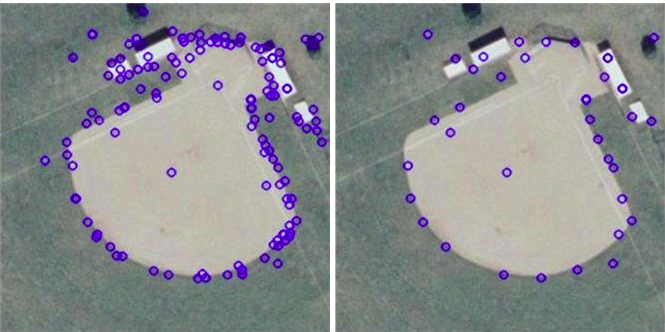
\includegraphics[width=0.45\textwidth]{images/v1survey/sift.png}
                      \caption{Scale-invariance feature transform}
                  \end{figure}
              }
        \item<3-> Action representation methods based on the trajectory of skeleton joints.
              % ThucTH
        \item<4-> Action representation based on human image sequences.
    \end{itemize}
\end{frame}


\begin{frame}{Handcrafted Action Features \\ (Depth, Skeleton)}
    Capture the human movements and spatial and temporal changes in video.
    \begin{itemize}
        \item Spatiotemporal volume-based action representation methods.

        \item STIP-based methods.
        \item Action representation methods based on the trajectory of skeleton joints.
        \item Action representation based on human image sequences.
    \end{itemize}
\end{frame}



